%description: Math 290 HW Template

%%%%% Beginning of preamble %%%%%

\documentclass[12pt]{article}  %What kind of document (article) and what size

%Packages to load which give you useful commands
\usepackage{subfig}
\usepackage{graphicx}
\usepackage{hyperref}
\usepackage{amssymb, amsmath, amsthm}

%Sets the margins

\textwidth = 6.5 in
\textheight = 9 in
\oddsidemargin = 0.0 in
\evensidemargin = 0.0 in
\topmargin = 0.0 in
\headheight = 0.0 in
\headsep = 0.0 in
\parskip = 0.2in
\parindent = 0.0in

%defines a few theorem-type environments
% \newtheorem{theorem}{Theorem}
% \newtheorem{corollary}[theorem]{Corollary}
% \newtheorem{definition}{Definition}

\newtheorem{definition}{Definition}
\newtheorem{example}{Example}
\newtheorem{fact}{Fact}
\newtheorem{remark}{Remark}
\newtheorem{theorem}{Theorem}
\newtheorem{proposition}{Proposition}
\newtheorem{lemma}{Lemma}
\newtheorem{corollary}{Corollary}

\renewcommand{\labelenumi}{\arabic{enumi}.}
\renewcommand{\labelenumii}{\arabic{enumi}.\arabic{enumii}.}
\renewcommand{\labelenumiii}{\arabic{enumi}.\arabic{enumii}.\arabic{enumiii}.}
\renewcommand{\labelenumiv}{\arabic{enumi}.\arabic{enumii}.\arabic{enumiii}.\arabic{enumiv}.}
\newlength{\alginputwidth}
\newlength{\algboxwidth}
\newcommand{\alginput}[1]{\makebox[1.5cm][l]{ {\sc Input:}} \parbox[t]{\alginputwidth}{{\it #1}}}
\newcommand{\algoutput}[1]{\makebox[1.5cm][l]{ {\sc Output:}} \parbox[t]{\alginputwidth}{{\it #1}}}
\newcommand{\algtitle}[1]{\underline{Algorithm \ {\bf #1}} \vspace*{1mm}\\}

%%%%% End of preamble %%%%%







\begin{document}

\title{Senior Project (draft)\\
Lafayette College \\
Department of Mathematics
}

\author{
{Wah Loon Keng}\thanks{
Lafayette College,
Easton, PA 18042, USA.
kengw{\tt @}lafayette.edu.}
% \qquad
% {Benjamin H. Draves}\thanks{
% Lafayette College,
% Easton, PA 18042, USA.
% dravesb{\tt @}lafayette.edu.}
      % \affaddr{Department of Computer Science}\\
%       \affaddr{Lafayette College}\\
%       \affaddr{Easton, PA 18042, USA}\\
%       \email{gexia@cs.lafayette.edu}
}
% \date{}
\maketitle


\begin{abstract}
We conduct a survey study on machine learning, its mathematical foundations, general techniques, and the latest progress in both the academia and the industry. However, most machine learners  excel only at the task they are trained for - this is a huge limitation. Motivated by this, we study a new paradigm called the Never-Ending Language Learning (NELL)$^{\ref{NELL}}$ and its potentials to overcome the singular nature of machine learners. Lastly, we design and implement a system based on NELL to predict the stock market performance. This is driven by the abundance of data, and the complex, interacting, non-singular nature of the task that a machine learner has yet to match a human on.
\end{abstract}


\clearpage
\tableofcontents
\clearpage






\section{Introduction} \label{intro}

We have just entered the golden age of machine learning. The field has in fact been around for decades, born from artificial intelligence and pattern recognition. It wasn't until recently that we have the level of computational power and the abundance of data to apply it. 

The machine learners have accomplished some truly astonishing feats. They are systems that are trained with a copious amount of data, which allows them to surpass the performance level of human experts. Today, they are actively being researched and deployed by the biggest tech companies such as Google, IBM, Microsoft, Facebook. In fact, their major products are powered by machine learning - Google Adsense, IBM Watson, and Facebook's M - doing tasks such as ads suggestion, image recognition, medical diagnosis, and natural language processing.

Typically, machine learning is best suited for the tasks that cannot be solved precisely or efficiently by algorithms. Many of these are what humans excel at - image recognition, language processing, pattern deduction. These capabilities are so trivial to us, yet they are so difficult to mimic by traditional algorithmic approaches. The prime example of {\em ``a child can easily recognize a cat in a picture, but a super computer can't''} best illustrates the failure of the algorithmic methods. Machine learning comes in to save the day.

In a nutshell, one can think of a it as a machine that ``learns'' from the data. On the implementation level, it is an automated regression software that can construct an impressively accurate model. The machine takes in a training set - input data where each entry is labeled with the intended output, then trains on it and learns to recognize the pattern. After that, when fed with new unlabeled input, it gives some predicted output based on its training. However, just like a typical regression model, its scope is strictly bounded to its training set. For example, a machine that recognizes cats cannot recognize a fish without extra training. Moreover, an image recognizer cannot diagnose diseases. In this sense a machine learner's scope is {\bf singular}. We will address this issue later.

The mathematical foundations of machine learning is built atop regression theory and linear algebra. Next, we present the formalization of a problem in machine learning as well as the terminologies.








\subsection{Formalization}

The following formalization is standard in the literature, we reference Tom M. Mitchell's popular textbook {\em Machine Learning}$^{\ref{Mitchell}}$.


\begin{definition}
A computer program is said to {\bf \em learn} from experience $E$ with respect to some class of tasks $T$ and performance measure $P$, if its performance at tasks in $T$, as measured by $P$, improves with experience $E$.
\end{definition}

We will use the terms {\em training} and {\em learning} interchangeably. Next, we define a {\bf problem}.

\begin{definition}
A {\bf \em problem} is a triple $\{T, P, E\}$. The goal of a machine learner solving the problem is to output a learned target function $\hat{V}$ that approximates an ideal target function $V$. The target function maps from the vector of input features $b$ to the set of output $O$.
\end{definition}


The experience $E$ represents the input data. It is the set of points specifying the configurations of the instances of the problem. To use it for training, the data must be {\em labeled / classified} - every input data must have its output. This is needed for the performance measure $P$. In the context, it is understood that the data is always labeled.

Often the data set is split into three parts - the training set, validation set, and test set, for obvious statistical reasons. The first is used to weight-tuning (see below) that may yield multiple candidates, the second for validating and choosing the best candidate, and the last for testing against new input data and detecting overfitters. 


The feature vector $b$, output $O$, and the function representation for $\hat{V}$ are defined by the programmer as deemed suitable. In a simple regression model, $b$ is a list of chosen input features, $O$ is the set of predicted values. Typically the target function $\hat{V}$ will include a set of weights $W = \{w_i \ | \ i \in \{1,2,\cdots,n\}\}$ which are tuned during the learning. They serve as the ``memory'' of the machine to compute predicted output once it is trained.



Upon having an explicit representation, and given the training data, we can devise the learning mechanism. First, define an error term $\mathcal{E}$ between the training data and the actual machine output. Then, use the error term to devise an algorithm that tunes the weights iteratively to minimize the error. The algorithm terminates on meeting a minimum threshold error, that is when the machine can perform sufficiently good.

\begin{example}
We provide an explicit example with the checkers game:

{\bf The checkers learning problem:}
\begin{enumerate}
\item Task $T$: playing checkers
\item Performance measure $P$: percent of games won
\item Training experience $E$: games played against another computer
\end{enumerate}

Next we need to determine the representations of the available knowledge. For the input feature vector $b$, we can choose a few board states, for instance, 
$$b = \langle x_1, x_2, x_3, x_4 \rangle$$
where the $x_i$'s are respectively the numbers of black pieces, black kings, red pieces and red kings on the board. We can choose a simple linear combination as our target function,
$$\hat{V}(b) = w_0 + w_1 x_1 + w_2 x_2 + w_3 x_3 + w_4 x_4$$
where $w_i$'s are the weights to be tuned during the training. Our output set $O$ is the list of moves at each game step given the features $x_i$'s at the time. We can define a bijection between the output range of $\hat{V}(b)$ and the $O$, but we will exclude it here.

Once we have a representation, devise a learning mechanism for training. Suppose now we have a set of positive (games won) training examples $\{\langle b, V_{train}(b) \rangle\}$. Define the error term using simple sum of squares $$\mathcal{E} = \sum_{\langle b, V_{train}(b) \rangle \in \ {\rm training\ examples}} (V_{train}(b) - \hat{V}_{train}(b))^2$$

Then, using this, devise an algorithm $A$ for training / weight-tuning. The error term above, when differentiated, yields gradient term of $\sim(V_{train}(b) - \hat{V}_{train}(b))$. One can imagine training as nodging a point closer to its true value, and the gradient gives the direction to nodge towards. This gives us a simple LMS algorithm for minimizing $\mathcal{E}$ using that gradient term:


\algtitle{LMS weight-tuning (learning) algorithm}
Initialize the weights $w_i$'s to random values. For each training example $\langle b, V_{train}(b) \rangle$:
\begin{enumerate}
	\item Use the current weights to compute $\hat{V}(b)$
	\item For each weight $w_i$, update it by $$w_i \leftarrow w_i + \eta \ (V_{train}(b) - \hat{V}_{train}(b)) \ x_i$$
\end{enumerate}

where $\eta$ is the parameter that moderates the stepsize. The algorithm terminates when $w_i$'s stop changing, i.e. when the error becomes sufficiently small (zero).

\end{example}

One can quickly see that the example machine learner above is just a simple regressor. Obviously this toy model will not be a good checker player. Nevertheless, given a huge training data, if we choose the right knowledge representation, feature vector $b$, target function $\hat{V}$, error term $\mathcal{E}$, and the learning algorithm, the resultant machine can perform very well. 

To suit a different type of problem, we can employ a different {\bf representation} - which we define to be the set $\{T, P, E, b, O\}$, as illustrated in Table \ref{rep}.



\begin{table}[h]
\begin{center}
\begin{tabular}{ | l | l | l || l | l | }

\hline
$T$ & $P$ & $E$ & $b$ & $O$ \\
\hline \hline
image recognition & correct labeling & labeled images & array of pixels & label of objects \\
\hline
driving a car & successful trip & test drives & traffic condition & wheel, pedals  \\
\hline
text translation & correct translations & pretranslated texts & semantics & translated text \\
\hline
ads suggestion & ads click rate & ads metadata & user profile & ads displayed \\
\hline
\end{tabular}
\caption{Different representations for various problems.}
\label{rep}
\end{center}
\end{table}



Moreover, we can employ different {\bf learning mechanisms} - which we define as the set of target function and learning algorithm, $\{\hat{V}, A\}$. This gives rise to the different techniques, or types, of machine learners such as the Neural Nets, Support Vector Machines, Deep Learning and etc. We will investigate the popular types in the next section.

A huge variety of machine learners today are being used for different purposes - most of the leading tech companies tweak and design their own. They may have very different {\bf representations} and {\bf learning mechanisms}, but the overall idea is still the same - gather labeled data, define the representations and learning algorithms, and train. The entire process is very modular, and the resultant machines are {\bf stagnant} - the machine no longer improve once training is done; and {\bf singular} - they can only function very narrowly only on the tasks they are trained for. For our discussions, we call this the {\bf stagnant \& singular paradigm}. In fact, this paradigm can readily be observed across most of the popular machine learners today. This will serve as the primary motivation of our work.









\subsection{Popular Techniques}

Before getting to the discussion on the paradigm, we take a quick look at the most common and powerful machine learners. These are derived from the same {\bf stagnant \& singular paradigm} by varying the {\bf representations} and {\bf learning mechanisms}.



\subsubsection{Decision Tree}

Decision tree is a popular method stemmed from artificial intelligence, used for hypothesis-searching and inductive reference. It uses a {\em tree representation}, where each node is a feature variable, and each edge is a value the feature takes on. The leaf nodes are the classification (output) values. Every path from the root to the leaf represents an instance of the feature $b$ and its output $o$. Moreover, different paths can be combined with logical $OR$ and $AND$ to yield a more general hypothesis space.

For the {\em learning mechanism}, a common method is to use the entropy measure and entropy gain while branching on each node (making a decision) while descending the tree. Suppose the data has $c$ classifications (e.g. $c=2$ for binary classifiers), the entropy is defined as $$Entropy(D) = \sum_{i=1}^{c} -p_i \ log_2 \ p_i$$ where $D$ is the data, $p_i$ is the proportion of samples of class $i$ in $D$. This allows us to judge the performance $P$ and search for the target function $\hat{V}$ by using the entropy gain for each feature $b$, $$Gain(D,b) = Entropy(D) - \sum_{v\in Values(b)} \frac{|D_v|}{D} Entropy(D_v)$$ where $D_v$ is the subset of D whose feature vector assumes the values equals to $v$.

Each path in the tree is a candidate hypothesis (collection of contributing features) to consider. Given the multitude of paths in the tree, the algorithm will end up with a set valid and consistent hypotheses. To resolve this, we simply use the {\bf Occam's razor} - choose the simplest hypothesis that fits the data. This will also prevent the initial overfitting.



\subsubsection{Artificial Neural Network (ANN)}

Often called just the ``neural net'', ANN was inspired by the biological system of neurons in the brain (note that it is inconsistent with the biological version). This is one of the earliest techniques, and has improved over the decades; the first practical usage was in the 80's, and today it is one of the most popular with countless variations. Here, we will describe the original and the most common designs.

Neural network is a practical method for learning examples that are real-valued, discretized, and multi-dimensional. It is so general that it has been applied successfully to image recognition, pattern-identification, robotics, speech and many more. Its popularity is primarily due to its power to learn accurately and its simplicity.

An ANN is a directed graph whose nodes are the feature variables, and edges are the weights. It is ordered into layers of nodes that are adjacently bipartite, i.e. every node in each layer connects (directionally) to all the nodes in the next layer. The first is called the {\em input layer}, the last the {\em output layer}, and the rest in between the {\em hidden layers}. A node is also called a {\em unit}, and those in the {\em hidden layers} are called {\em hidden units.}

The {\em input layer} corresponds to the feature vector $b$ - each unit takes the value for each feature variable. Similarly the output layer corresponds to the output $o$. Each iteration of training involves a series of computation from the input, through the hidden layers, to the output. Across the net, the outputs become the inputs for the next layer.

Suppose we have at layer $i$ indexed nodes $x_{i,1}, x_{i,2}, \cdots, x_{i,p}$ bipartite to nodes $x_{i+1,1}, x_{i+1,2}, \cdots, x_{i+1,q}$ at layer $i+1$. We can simply represent as the edges with their weights with subscript indicating the connection. For example, the first node $x_{i,1}$ connects to all the edges in the next layer via $w_{i,1,1}, w_{i,1,2}, \cdots, w_{i,1,q}$.

Then, we can define the function for mapping input values at $x_{i,1}, x_{i,2}, \cdots, x_{i,p}$ to an output value at $x_{i+1,j}$, i.e. we can define a target function for an output node $x_{i+1,j}$ $$\hat{V}_{i+1,j} : \{ w_{i,1,j}, w_{i,2,j}, \cdots, w_{i,p,j} \} \times \{ x_{i,1}, x_{i,2}, \cdots, x_{i,p} \} \mapsto x_{i+1,j}$$

Typically, an inner product is sufficient to yield a good ANN. For this we have the form $$\hat{V}_{i+1,j} = \langle  w_{i,1,j}, \cdots, w_{i,p,j}  \rangle \cdot \langle  x_{i,1}, \cdots, x_{i,p}  \rangle = w_{i,1,j}x_{i,1} + \cdots + w_{i,p,j}x_{i,p}$$

\begin{figure}
\centering
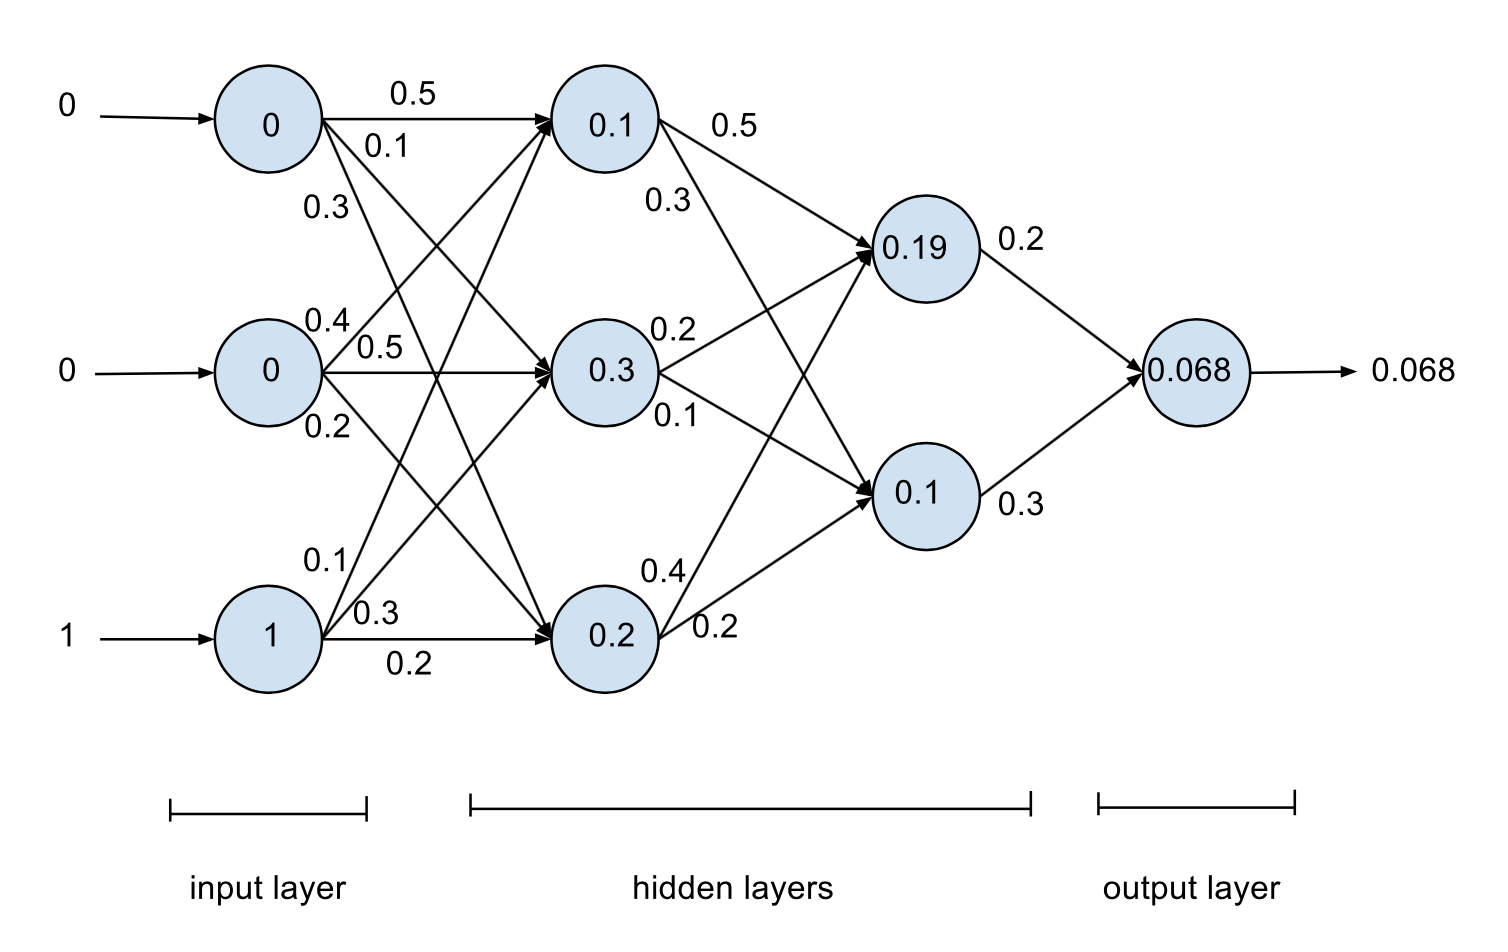
\includegraphics[scale=0.5]{images/ANN.png}\\
\caption{An ANN with 3 input units, 2 hidden layers each with 3 and 2 hidden units, and 1 output unit. The target function is the dot product between the incident values from the previous layer and their edge weights.}\label{ANN-fig}
\end{figure}

An explicit example is provided in Figure \ref{ANN-fig}. The feature vector input is $b = \langle 0,0,1 \rangle$; the value $$x_{2,1} = \hat{V}_{2,1} = w_{1,1,1}x_{1,1} + w_{1,2,1}x_{1,2} + w_{1,3,1}x_{1,3} = 0.5 \cdot 0 + 0.4 \cdot 0 + 0.1 \cdot 1 = 0.1$$

If we wish, we can define the target function $\hat{V} : b \mapsto o$ for the entire ANN by taking the ordered composition of the sub-target functions defined above, but this is cumbersome. Often the graph representation is used.

We can create variations of ANN by tweaking the target function $\hat{V}$, the error term $\mathcal{E}$, and the training algorithm $A$. Moreover, we can change the graph structures by adding more hierarchies (convolutional, deep learning) or {\em backedges} to create cycles (recurrent neural network RNN).

With data $\{\langle b, V(b) \rangle\}$, the training goes as usual. A single iteration of training starts from the input layer and ends at the output layer. The error term is then used with the tuning algorithm $A$ to tune the edge weights, i.e. use the errors to update the weights. Reiterate the process until the output error is smaller than a threshold. Unsurprisingly, training a large neural net can take up to months, but the results can be very impressive. Below, we describe some of the most powerful versions that have recently made the news.





\subsubsection{ANN with Perceptrons}

Given the general design above, we can simplify our notations to aid discussions. Focusing on a subnetwork, look at a single output unit $o$ with incoming inputs $x_1, x_2, \cdots, x_k$ and weights $w_1, w_2, \cdots, w_k$, the target function for a perceptron unit is
\[
o(x_1, \cdots, x_k) =
\begin{cases}
1 &\text{if } w_0 + w_1 x_1 + w_2 x_2 + \cdots + w_k x_k > 0\\
-1 &\text{otherwise }
\end{cases}
\]

Concisely, we write $$o(\vec{x}) = sign(\vec{w} \cdot \vec{x})$$

The training rule for the algorithm is a simple update, $$w_i \leftarrow w_i + \eta(t-o)x_i$$ where $\eta$ is the stepsize moderation called the {\em learning rate}, $t$ is the target output value, $o$ the actual perceptron output, $x_i$ the input node value.




\subsubsection{ANN with Gradient Descent}

The gradient descent can be seen as a refinement to the perceptron. Its target function is $$o(\vec{x}) = \vec{w} \cdot \vec{x}$$

The unit is called a {\em linear unit} for an obvious reason. The error term is defined as $$\mathcal{E}(\vec{w}) = \frac{1}{2} \sum_{d \in D} (t_d - o_d)^2$$ where $D$ is the data, $t_d$ is the target output value, $o_d$ the unit output for a data point $d$. This will guide the weight-tuning rule for the algorithm, which also gives its name.

Given the formalism, we can equivalently view as a vector space. Our task then is to find the set of weights that yields the right target function. Minimizing the error term is then equivalent to minimizing the error surface in the vector space. We know this is done by stepping in the direction of the steepest descent along the error surface, which is simply the gradient of the error term $$\nabla \mathcal{E}(\vec{w}) =\ \langle  \frac{\partial \mathcal{E}}{\partial w_0}, \frac{\partial \mathcal{E}}{\partial w_1}, \cdots, \frac{\partial \mathcal{E}}{\partial w_k}  \rangle$$

Then, the tuning rule is simply $$\vec{w} \leftarrow \vec{w} - \eta \nabla \mathcal{E}(\vec{w})$$ where $\eta$ is the learning rate. When written in component form we get $$w_i \leftarrow w_i - \Delta w_i = w_i - \eta \frac{\partial \mathcal{E}}{\partial w_i}$$


\algtitle{Gradient-Descent(Data, $\eta$)}
Each training example $d \in Data$ is of the form $d = \langle \vec{x}, t \rangle$, where $\vec{x}$ is the input vector, $t$ the target output value, $\eta$ the learning rate. Note that the partials are found using discretized iterations at step 2.2.2.

\begin{enumerate}
	\item Initialize the weights $w_i$'s to small random values.
	\item Until termination condition (defined separately), do
		\begin{enumerate}
			\item Initialize each $\Delta w_i$ to 0
			\item For each $\langle \vec{x}, t \rangle \in Data$, do 
			\begin{enumerate}
				\item Input $\vec{x}$ and computer output $o$
				\item For each unit weight $w_i$, do $$\Delta w_i \leftarrow w_i + \eta(t-o)x_i$$
			\end{enumerate}
			\item For each linear unit weight $w_i$, do $$w_i \leftarrow w_i + \Delta w_i$$
		\end{enumerate}
\end{enumerate}





\subsubsection{ANN with Backpropagation}

The invention of {\em Backpropagation} reinvigorated ANN after its loss of popularity due to practical limitations. First, we improve the target function by using a sigmoid (logistic) function, yielding a {\em sigmoid unit} $$o = \sigma (\vec{w} \cdot \vec{x})$$ where $$\sigma(y) = \frac{1}{1+e^{-y}}$$ It has some very nice properties. The function maps the entire real domain into $(0,1)$; it increases monotonically; it is smooth with a convenient derivative $\sigma'(y) = \sigma(y) (1 - \sigma(y))$, which is computationally cheap.

Next, {\em Backpropagation} can efficiently train a large multilayer network. We can directly generalize the error term as the sum over all nodes at a layer, $$\mathcal{E}(\vec{w}) = \frac{1}{2} \sum_{d \in D} \sum_{k \in outputs} (t_{d,k} - o_{d,k})^2$$

The following algorithm constructs an ANN that uses {\em Backpropagation} with the number of units as parameters.


\algtitle{Backpropagation(Data, $\eta$, $n_{in}$, $n_{out}$, $n_{hidden}$)}
Each training example $d \in Data$ is of the form $d = \langle \vec{x}, t \rangle$, where $\vec{x}$ is the input vector, $t$ the target output value, $\eta$ the learning rate. $n_{in}$, $n_{out}$, $n_{hidden}$ are respectively the numbers of units in the input, hidden and output layers. Double indices are ordered as {\em from, to}. Note that the partials are found using discretized iterations at step 3.1.2.

\begin{enumerate}
	\item Create a feed-forward network with $n_{in}$ inputs, $n_{hidden}$ hidden units, and $n_{out}$ output units.
	\item Initialize all weights to small random values.
	\item Until termination condition (defined separately), do
		\begin{enumerate}
			\item For each $\langle \vec{x}, t \rangle \in Data$, do:
			\begin{enumerate}
				\item (Propagate the input through the network) Input $\vec{x}$ and computer output $o$ for every unit
				\item (Propagate the errors backward through the network) For each output unit $o_k$, compute its error term $\delta_k$ by $$\delta_k \leftarrow o_k(1-o_k)(t_k-o_k)$$
				\item For each hidden unit $h$, compute its error term $\delta_h$ by $$\delta_h \leftarrow o_h(1-o_h)\sum_{k \in outputs}w_{hk}\delta_{k}$$
				\item Update each weight $w_{ij}$ by $$w_{ij} \leftarrow w_{ij} + \Delta w_{ij}$$ where $$\Delta w_{ij} = \eta \ \delta_j \ x_{ij}$$
			\end{enumerate}
		\end{enumerate}
\end{enumerate}


There are obvious caveats to {\em Backpropagation}, namely convergence and local minima. The former can be resolved by added heuristics in the externally-defined termination condition; the latter can be overcome by updating the algorithm with {\em stochastic gradient descent} instead. Fortunately for most practical purposes, these limitations can safely be ignored.

This ANN is in fact so powerful that it can represent every Boolean function, approximate any continuous functions, as well as arbitrary functions. The famous {\em Universal Approximation Theorem}$^{\ref{Cybenko}}$ states that a feedforward ANN with three layers of units can achieve this generality.

Since its invention in the 80's it has become the primary method for ANN. Indeed thus far in this paper, {\em Backpropagation} is the most powerful machine learner, until the recent rise of the more powerful {\em Deep Learning.}



\subsubsection{ANN with Deep Learning}







performance, 3 layers few units suff to approx most functions?

Each round of training takes the input 


Input layers X
output layers
recursive propagation
T, P, E, b, O
V, A


\subsubsection{SVM}

\subsection{Applications}
Google translate
google ad sense
google deep dream, deep mind
Google deep learning (play game!)
IBM watson


\subsection{Paradigm: Powers \& Limitations}



\section{NELL as a New Paradigm}

\subsection{Inspiration \& Features}
\subsection{Architecture}
\subsection{Applications}
\subsection{Powers \& Limitations}



\section{NELL for Stock Market Prediction}

\subsection{Problem statement}
\subsection{Potential of NELL}
\subsection{Design}
\subsection{Implementation}
\subsection{Assessment}


\section{Future Work}






\subsection{Results, Performance, and Analysis }
We immediately see several trends given by the fun function. A clear player order effect was found between nearly every AI. While some AI’s were simply more powerful and able to win regardless of characteristics, in nearly every case we see that more wins are generated from the AI if they play first compared to when they play second. For some more closely related AI’s, the odds of winning changes in its favor given the player order effect. From this we can conclude that for certain comparable AI’s, player order may greatly affect the outcome of the game. 

Furthermore, in every case, the trend line from the total army plot simply shifted its intercept value but held consistent slope. This intercept can be credited to first round play. After the first round (when the first point is calculated) the army advantage can be a one player advantage. This first round however rarely changes the results of the game. Consider figure 1. 

\begin{center}
% \includegraphics[scale=0.6]{images/Figure_1.jpg}\\
{\footnotesize Figure 1.}
\end{center}

Here the green and red dots represent AI0’s and AI4’s percent total armies respectively over time. Again, the dots only represent games in which a definitive winner was found. Here we see that AI0 has a clear advantage but when the player order is changed, AI4 wins more games. Notice, however, while the trend line shifts down, that the slope stays constant. This implies that while the game is certainly affected by player order, on average, the game develops the same regardless of player order. 

For the same AI match, the fun function provides two survival charts. Now consider figure 2. 


\begin{center}
% \includegraphics[scale=0.6]{images/Figure_2.jpg}\\
{\footnotesize Figure 2.}
\end{center}

In the first plot we see that player two holds several armies until near round 50. Suddenly over the next two rounds however, we see an incredible drop off. AI0 has mostly defensive characteristics. From this it appears that AI0 condenses its portion of the graph and builds armies. Somewhere near halfway through the game, it branches out and gains several territories in a very small period of time. When the order of the game is reversed we see a much more even trend. Both AI’s seem to lose armies at a consistent rate. This effect could be accredited to player order effect or the characteristics of the players in regards to their section of the sub graph. 


While these trends, in general, hold true, one AI in particular defied the general trends. We will call this AI, AI3. AI3, in general, tended to produce more wins when playing in the second player position. This trend was tested more rigorously against 15 new AI’s. From this data, the fun function produced the win records for both AI3 and the other AI’s for both player order. The difference between wins was then calculated. That is $\Delta \emph{win} = \emph{AI3\_wins} - \emph{AIOpponent\_wins}$. This figure was calculated for both player orders. This data is represented in figure 3.



\begin{center}
% \includegraphics[scale=0.6]{images/Figure_3.jpg}\\
{\footnotesize Figure 3.}
\end{center}


As in figure 3, on average AI3 wins 3.625 games while playing second in comparison to playing first where the AI won only 0.5 games on average. This in turn would seem to offer a solution to the player order effect, mentioned above. By simply playing the AI3 characteristics (“Survival”, “Defensive”, “Cautious”, “Carry”), on average the advantage would go to the second player, thus making player order obsolete. 


Another nuanced observation shows that this conclusion may not be entirely true. Under further observation, another AI which we will call AI4 (“Survival”, “Aggressive”, “Tactical”, “Rusher”) seemed to be superior to AI3 in both player orders. A more rigorous study of these two AI’s revealed that the assumption was correct. The fun function showed that on average, AI4 wins more often than AI3. Consider figure 4 and figure 5. 



\begin{center}
% \includegraphics[scale=0.6]{images/Figure_4.jpg}\\
{\footnotesize Figure 4.}\\
% \includegraphics[scale=0.6]{images/Figure_5.jpg}\\
{\footnotesize Figure 5.}
\end{center}

Notice that these two figures show very low correlation when player order changes. When AI3 goes first, it grosses more wins than AI4. When AI3 goes second, however, AI4 wins the majority of the games. While by a narrow margin, when AI4 goes first, AI4 wins 56 more games than AI3 in a 500 game trial. Thus if AI3 plays second they will on average lose to AI4. 


\subsection{AI behaviors and Surprises}
In this project several AI’s were posed against each other in a game of Risk. Initially, it was predicted that a large player order effect would affect the game. This hypothesis held true for the majority of AI’s that were tested in this experiment. AI3 however, proved that by using the correct strategy, a player would actually hold an advantage by going second in the game. From this however, AI4 proved that their still exist AI’s that can beat AI3 while being the first player to move. 

From this project, we advise future Risk players to abstain from declaring their player strategy until the player order is determined. From this, we advise that second players play a cautious, defensive game, while first players play with aggressive tendencies. A consistent analysis of strategy will reveal the best strategy for either player to take throughout the duration of the game. 



\section{Conclusion}
We have reformalized the board game \emph{Risk} as a graph optimization, and implemented an AI to solve the problem, i.e. to play the game. Several decision algorithms were devised based on graph properties, and they in turn form the personalities of the AI. Our study of 4 binary traits, or a total of 16 personality variations of the AI, is merely the beginning. We have discovered some interesting AI behaviours and performance at a level beyond any human players. One can potentially investigate even more variations of the traits.

For future studies, an analysis of subgraphs would provide deep insight into the value of individual territories. The AI’s are built in such a way that the priority function is based off of current demographic of troops and shape of their graph. Evaluating the graph as a whole would provide insight to the value of different subgraphs that would proactively affect the priority function. This conditional thinking is much more like the ideas of a human player and thus could inform future strategies. 

Furthermore, game shifts could be analyzed using the fun function and the aforementioned subgraph analysis. This would allow for defensive players an understanding of which territories that are worth defending and worth conceding. This shift parameter would allow for insight to game length, army distribution, and other key factors.  





\section{References}


\begin{enumerate}

\item Carnegie Mellon University, \emph{NELL: Never-Ending Language Learning}. \url{http://rtw.ml.cmu.edu/rtw/}\label{NELL}

\item Tom M. Mitchell, \emph{Machine Learning}. McGraw-Hill, 1997.\label{Mitchell}

\item Cybenko., G. (1989) \emph{Approximations by superpositions of sigmoidal functions}, Mathematics of Control, Signals, and Systems, 2 (4), 303-314. \label{Cybenko}


\end{enumerate}



\end{document} 

